\documentclass[oneside,a4paper,14pt]{extarticle}

\usepackage[russian]{babel}
\usepackage{fontspec}
\setmainfont{Times New Roman}
\setmonofont{Courier New}
\usepackage[
	a4paper,
	top=2cm,
	bottom=2cm,
	left=2.5cm,
	right=1.5cm
]{geometry}
\usepackage{textcomp}
\usepackage{indentfirst}
\usepackage{listings}
\usepackage{xcolor}
\usepackage{enumitem}
\usepackage{graphicx}
\usepackage{caption}
\usepackage{amsmath}
\usepackage{float}
\usepackage{titlesec}
\usepackage{hyperref}

\titleformat{\section}{\normalsize\bfseries}{\thesection}{1em}{}
\titleformat{\subsection}{\normalsize\bfseries}{\thesubsection}{1em}{}
\titleformat{\subsubsection}{\normalsize\bfseries}{\thesubsubsection}{1em}{}

\renewcommand\baselinestretch{1.33}\normalsize
\setlength{\parindent}{1.25cm}

\renewcommand{\lstlistingname}{Листинг}
\lstset{
	basicstyle=\ttfamily\small,
	keywordstyle=\color{blue},
	commentstyle=\color{green!60!black},
	stringstyle=\color{red},
	numbers=left,
	numberstyle=\tiny\color{gray},
	frame=single,
	breaklines=true,
	showstringspaces=false,
	tabsize=2,
	inputencoding=utf8,
	extendedchars=true,
	literate={·}{{\hspace{0.35em}}}1,
	captionpos=t,
	xleftmargin=1em
}

\begin{document}

\newpage
\thispagestyle{empty}
\begin{center}
	МИНИСТЕРСТВО НАУКИ И ВЫСШЕГО ОБРАЗОВАНИЯ\\
	РОССИЙСКОЙ ФЕДЕРАЦИИ
	ФЕДЕРАЛЬНОЕ ГОСУДАРСТВЕННОЕ БЮДЖЕТНОЕ\\
	ОБРАЗОВАТЕЛЬНОЕ
	УЧРЕЖДЕНИЕ ВЫСШЕГО ОБРАЗОВАНИЯ\\
	«ВЯТСКИЙ ГОСУДАРСТВЕННЫЙ УНИВЕРСИТЕТ»\\
	Институт математики и информационных систем\\
	Факультет автоматики и вычислительной техники\\
	Кафедра электронных вычислительных машин
\end{center}

\vspace{20mm}

\begin{center}
	Отчёт по лабораторной работе №5\\
	по дисциплине\\
	<<Программирование>>
\end{center}

\vspace{48mm}

\noindent
Выполнил студент гр. ИВТб-1303-06-00 \hfill \rule[-0,5mm]{30mm}{0.15mm}\,/Шубин В. Ю./
\newline
Проверил преподаватель кафедры ЭВМ \hfill \rule[-0,5mm]{30mm}{0.15mm}\,/Баташев П.А./

\vfill

\begin{center}
	Киров\\
	2026
\end{center}

\newpage
\thispagestyle{empty}

\section*{Цель работы}
Изучить методы обработки данных, которые не помещаются в оперативную память, на примере внешней сортировки больших CSV-файлов. Закрепить навыки реализации двухфазного алгоритма «разбиение -- слияние» на языках C++ и Python, провести сравнительный анализ и создать графическое приложение для демонстрации работоспособности обеих реализаций.

\section*{Постановка задачи}
Предметная область сохранена прежней: каждая строка файла описывает студента и содержит шесть полей, разделённых запятой:
\begin{itemize}[leftmargin=*]
	\item \texttt{name} --- фамилия и имя (до 63 байт в UTF-8);
	\item \texttt{group} --- обозначение учебной группы (до 39 байт);
	\item \texttt{dob} --- дата рождения в формате \texttt{YYYY.MM.DD};
	\item \texttt{height} --- рост в сантиметрах (целое 32-битное число);
	\item \texttt{weight} --- вес в килограммах (число с плавающей точкой);
	\item \texttt{expulsion} --- признак нахождения в списке на отчисление.
\end{itemize}

В бинарном представлении C++ использует упакованную структуру из 129 байт. Требуется:
\begin{itemize}[leftmargin=*]
	\item генерировать файл \texttt{data.csv} размером более 1~ГБ;
	\item сортировать его в \texttt{sorted.txt} по любому из шести полей и в любом направлении;
	\item ограничить потребление ОЗУ 10\,\% от размера исходного файла;
	\item удалить временные файлы после завершения;
	\item оценить время разбиения и слияния и уложиться в 10~минут;
	\item обеспечить генерацию, выбор файла и просмотр фрагментов через GUI.
\end{itemize}

Итоговое приложение \texttt{lab5.exe} собрано в один исполняемый файл средствами PyInstaller; DLL сортировки C++ извлекается во временный каталог приложения и загружается оттуда.

\section*{Описание алгоритма}
Используется классическая схема внешней сортировки с двумя фазами. Размер сортируемого блока адаптируется к размеру исходного файла, поэтому ограничение памяти соблюдается и на файлах, которые только немного превышают 1~ГБ, и на больших файлах.

\subsection*{Фаза разбиения}
\begin{itemize}[leftmargin=*]
	\item C++ читает файл блоками по 10~МиБ и откатывает позицию к последнему символу \texttt{LF}, чтобы не разорвать CSV-запись.
	\item Python использует \texttt{csv.reader} и накапливает до 120~тысяч строк или до 8~млн символов в одном блоке.
	\item Накопленные записи сортируются по выбранному ключу: в C++ --- \texttt{std::sort}, в Python --- встроенный \texttt{list.sort}.
	\item Каждый отсортированный блок сохраняется в отдельный временный файл: \texttt{.lab5\_cpp\_tmp\_PID} или \texttt{.lab5\_py\_tmp\_PID} рядом с исходным файлом.
\end{itemize}

\subsection*{Фаза слияния}
\begin{itemize}[leftmargin=*]
	\item Из всех временных файлов берётся по первой записи и формируется приоритетная очередь.
	\item В C++ применяется \texttt{std::priority\_queue}, в Python --- \texttt{heapq}. Для убывания используется обёртка ключа с инвертированным оператором сравнения.
	\item На каждом шаге из очереди извлекается нужная запись, записывается в \texttt{sorted.txt}, а из её исходного файла берётся следующая запись.
	\item Вывод буферизуется (C++ --- 10~МиБ), после чего временный каталог удаляется.
\end{itemize}

\begin{figure}[H]
	\centering
	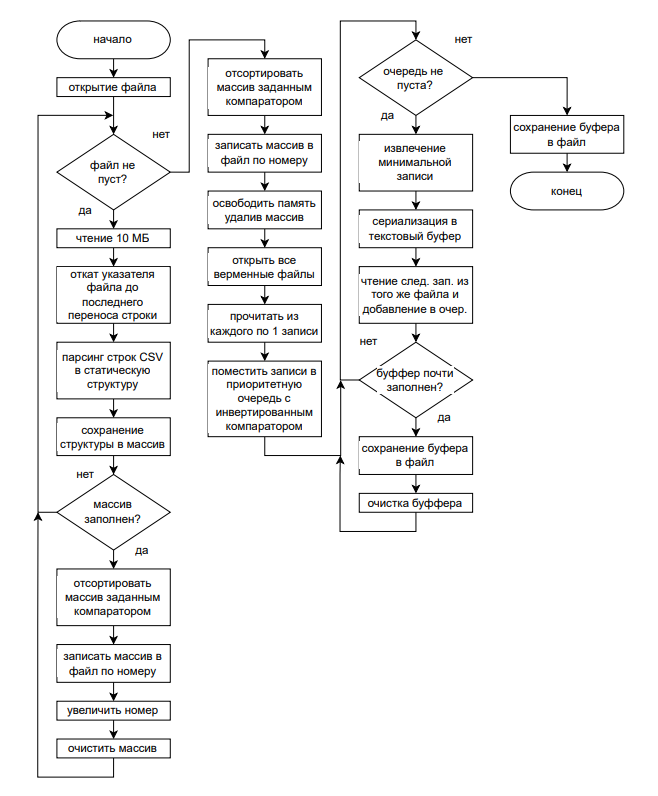
\includegraphics[width=\textwidth,height=0.82\textheight,keepaspectratio]{1.png}
	\caption{Схема алгоритма внешней сортировки}
\end{figure}

\section*{Сравнение реализаций C++ и Python}
\subsection*{Общая схема}
Обе реализации используют одинаковую логику разбиения и $K$-образного слияния. Различия связаны главным образом с языковыми средствами: C++ работает с плотной бинарной структурой и указателями, Python --- с текстовыми строками, модулем \texttt{csv} и динамическими объектами.

\begin{table}[H]
	\centering
	\caption{Сопоставление двух реализаций}
	\renewcommand{\arraystretch}{1.2}
	\begin{tabular}{|p{3.6cm}|p{6.0cm}|p{6.2cm}|}
		\hline
		Характеристика & C++ & Python \\
		\hline
		Файловый ввод-вывод & \texttt{fstream}, бинарные блоки & \texttt{with open(...)} и модуль \texttt{csv} \\
		\hline
		Представление записи & Упакованная структура \texttt{Record} (129~байт) & Список из шести строк \\
		\hline
		Размер блока & До 300\,000 записей, адаптивно & До 120\,000 строк или 8~млн символов \\
		\hline
		Сортировка блока & \texttt{std::sort} & \texttt{list.sort} \\
		\hline
		Слияние & \texttt{std::priority\_queue} & \texttt{heapq} \\
		\hline
		Временные файлы & Бинарные \texttt{.tmp} в отдельном каталоге & Текстовые CSV-файлы в отдельном каталоге \\
		\hline
	\end{tabular}
\end{table}

\subsection*{Причины различий в производительности}
C++ быстрее, потому что разбор строки выполняется указателями, записи имеют фиксированный размер, а сравнение ключей компилируется в нативный код. Python тратит больше времени на создание строковых объектов, вызовы \texttt{csv.reader}/\texttt{csv.writer} и сравнения в куче. Тем не менее оба варианта удовлетворяют требованию времени сортировки.

Ограничение памяти достигается за счёт адаптивного размера блока. В C++ при файле 1,1~ГБ блок содержит не более 300\,000 записей по 129~байт, то есть около 37~МиБ, плюс два буфера по 10~МиБ. В Python одновременно обрабатывается не более 120\,000 строк; пиковое потребление по результатам замера составило 80,8~МиБ, что меньше 10\,\% от 1,1~ГБ.

\subsection*{Обработка ошибок и интерфейс}
Модуль C++ предоставляет расширенную функцию \texttt{external\_sort\_ex}, которая возвращает булево значение и передаёт в GUI строку с временами этапов. Старый вызов \texttt{external\_sort} оставлен для обратной совместимости. Все обновления Tkinter выполняются через очередь событий \texttt{after}, поэтому работа сортировки в отдельном потоке не нарушает потокобезопасность интерфейса.

GUI позволяет сгенерировать файл заданного объёма (по умолчанию 1100~МиБ), выбрать файл, выбрать модуль C++ или Python, ключ и направление сортировки, просмотреть заданный участок исходного или отсортированного файла, а также автоматически проверить порядок ключей в \texttt{sorted.txt}. Времена разбиения, слияния и общее время выводятся в текстовую область окна.

\section*{Анализ результатов}
Эксперимент проводился на сгенерированном файле \texttt{data.csv} размером 1\,153\,433\,605~байт (1100~МиБ, 15\,392\,410~записей). Сортировка выполнялась по полю «Группа» по возрастанию. Результат проверен построенным сканированием отсортированного файла; временные каталоги после завершения отсутствуют.

\begin{table}[H]
	\centering
	\caption{Результаты сортировки файла 1100~МиБ}
	\renewcommand{\arraystretch}{1.2}
	\begin{tabular}{|p{4.0cm}|p{5.5cm}|p{5.5cm}|}
		\hline
		Показатель & C++ & Python \\
		\hline
		Разбиение, с & 35.63 & 116.85 \\
		\hline
		Слияние, с & 23.19 & 135.12 \\
		\hline
		Общее время, с & 58.92 & 251.98 \\
		\hline
		Пиковое потребление ОЗУ, МиБ & 60.4 & 80.8 \\
		\hline
		Доля от размера файла & 5.2\,\% & 7.0\,\% \\
		\hline
	\end{tabular}
\end{table}

Обе реализации укладываются в ограничение 10~минут и 10\,\% памяти. C++ примерно в 4,3 раза быстрее Python в основном за счёт бинарного представления записей и более дешёвых сравнений. В Python наибольшие затраты приходятся на разбор CSV-строк и работу кучи при слиянии.

\section*{Выводы}
В ходе работы реализована внешняя сортировка CSV-файла, размер которого превышает объём оперативной памяти, выделенной под алгоритм. Созданы два вычислительных модуля --- на C++ и Python --- и единое приложение \texttt{lab5.exe}, объединяющее генерацию данных, сортировку, вывод времен, просмотр и проверку результата.

Основные результаты:
\begin{itemize}[leftmargin=*]
	\item генератор создаёт корректный CSV-файл размером более 1~ГБ и работает повторно;
	\item сортировка поддерживает все шесть ключей и оба направления;
	\item память ограничена адаптивным размером блока и не превышает 10\,\% от исходного файла;
	\item временные файлы создаются в отдельных каталогах и удаляются после сортировки;
	\item время сортировки обоих модулей меньше 10~минут;
	\item GUI отображает времена этапов и позволяет проверить правильность результата.
\end{itemize}

Наиболее быстрой является реализация на C++, однако Python-версия проще в сопровождении и полностью соответствует требованиям методички по использованию менеджеров контекста и библиотеки \texttt{csv}. Полученные подходы применимы к обработке больших наборов данных, не помещающихся в оперативную память.

\newpage
\section*{Листинги кода}

\lstinputlisting[caption={Код модуля сортировки на C++}]{listings_src/external_sort.cpp}

\lstinputlisting[caption={Заголовочный файл для модуля на C++}]{listings_src/external_sort.h}

\lstinputlisting[caption={Код модуля сортировки на Python},language=Python]{listings_src/external_sort.py}

\lstinputlisting[caption={Код генератора тестовых данных},language=Python]{listings_src/generate.py}

\lstinputlisting[caption={Код приложения с пользовательским интерфейсом},language=Python]{listings_src/main.py}

\end{document}
